\documentclass[12pt,a4paper]{article}
\usepackage[utf8]{inputenc}
\usepackage[czech]{babel}
\usepackage{datetime}
\usepackage{tabularx}
\usepackage{graphicx}
\usepackage[colorlinks=true,linkcolor=blue,urlcolor=green]{hyperref}
\renewcommand{\dateseparator}{. }
\begin{document}

\title{Problém batohu hrubou silou a jednoduchou heuristikou}
\author{Dominik Plíšek}
\date{\dmyyyydate\today}
\maketitle

\section*{Úvod k implementaci}

Rozhodl jsem se pro implementaci v jazyce C, jelikož mám rád u podobných algoritmů pod svoji kontrolou paměťové nároky. 
Napsal jsem obecné struktury pro:

\begin{description}
\item[instanci problému] id, kapacita, počet věcí a pole věcí
\item[řešení problému] váha, cena, bitová mapa značící přítomnost věcí z instance v batohu
\item[věci v batohu] váha, cena
\end{description}

Napsal jsem obecnou $main()$ metodu
pro řešení instancí ze $stdin$ a výpis výsledků do $stdout$. Vytvořil jsem si hlavičku funkce pro obecné řešení instance
problému. Implementaci této funkce v jednotlivých způsobech řešení zaměňuji.

Výpočet provádělo jedno vlákno čtyřjádrového procesoru 2,3 GHz Intel Core i7 s 6 MB L3 cache.
Naměřené časy představují procesorový čas, tedy čas, kdy skutečně vlákno pracovalo.


\section{Hrubou silou}

Naprogramujte řešení problému batohu hrubou silou (tj. exaktně). Na zkušebních datech pozorujte závislost výpočetního času na n.

\subsection{Diskuse}

Řešení hrubou silou znamená vyzkoušet všechny stavy stavového prostoru, abychom se 100\% jistotou nelezli nejlepší (nebo jedno
z nejlepších) řešení.

Je možno jej implementovat buď iterativně, nebo rekurzivně. Iterativní metoda by v tom případě byla asi přehlednější,
ale vzhledem k tomu, že úlohy, které budou následovat, bude patrně podstatně snažší řešit rekurzí, 
použil jsem rekurzi i pro hrubou sílu.

\subsection{Implementace}

Program rekurzivně volá funkci se zvětšujícím se indexem, která vždy zkusí věc s daným indexem do batohu
přidat i nepřidat, načež zavolá dvakrát sama sebe, aby zkusila, co se bude dít v obou případech. Program věc do batohu
nepřidá v případě, že se do něj již nevejde. Takto postupně vyzkouší všechny kombinace věcí v batohu. Nakonec
vrátí výsledné tvrzení o nejvyšší možné ceně a jak jí dosáhnout.

Velmi hrubá kostra:

\begin{verbatim}
vyřešInstanci(instance) {
  vyhodnoťStavVýsledku(výsledek, 0)
  vrať výsledek
}

vyhodnoťStavVýsledku(výsledek, index) {
  nejsou-li již věci, vrať se
  vejde-li se věc s indexem do batohu (výsledku),
    pak si zapamatuj výsledek,
    dej ji tam 
    a vyhodnoťStavVýsledku(výsledek, index)
  pak zkus vyhodnotitStavVýsledku(původníVýsledek, index)
    -- bez této věci
  byla-li první možnost výhodnější, vrať se k ní
}
\end{verbatim}

\subsection{Výsledky}

Závislost času výpočtu na počtu věcí k přibalení do batohu je vidět z této tabulky:

\begin{center}
\begin{tabular}{|c|c|}
\hline
Počet věcí & Čas výpočtu (millis) \\
\hline\hline
4 & 0.520 \\
\hline
10 & 14.634 \\
\hline
15 & 709.653 \\
\hline
20 & 21424.700 \\
\hline
22 & 77237.619 \\
\hline
25 & 648182.280 \\
\hline
\end{tabular}
\end{center}

Pro lepší představu, jak rychle čas roste, přidávám proložený graf:

\begin{center}
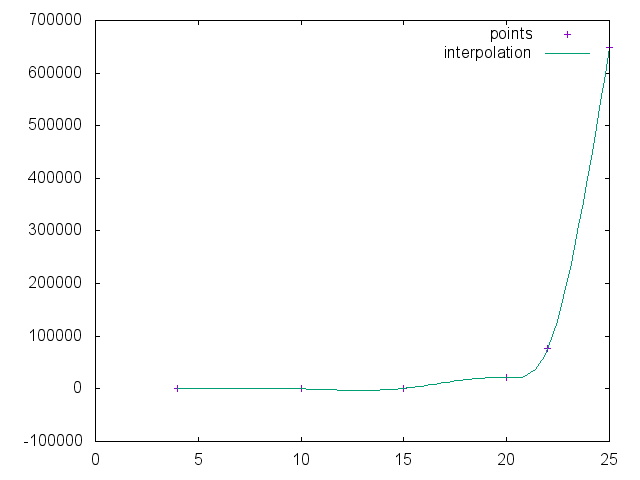
\includegraphics[width=\textwidth]{brute}
\end{center}



\section{Jednoduchou heuristikou}

Naprogramujte řešení problému batohu heuristikou podle poměru cena/váha. Pozorujte
\begin{itemize}
\item závislost výpočetního času na n. Grafy jsou vítány (i pro exaktní metodu).
\item průměrnou a maximální relativní chybu (tj. zhoršení proti exaktní metodě)
\end{itemize}

\subsection{Diskuse}

Řešení se liší od hrubé síly především v tom, že se v každém kroku vyzkouší pouze jedna možnost, nikoli dvě.
To znamená, že prostor řešení se prochází lineárně.

\subsection{Implementace}

Program opět rekurzivně volá funkci, která přidává věci do batohu.
Tentokrát ale nepoužívá index, protože věc, kterou do batohu přidá, v každém kroku vybírá podle heuristiky.
Konkrétně vždy spočítá poměr cena/váha a vybírá věc s nejvyšším.

Jakmile vybere věc, která se přidá, už ji neodebere. Považuje výběr za rozhodnutý a vstupuje 
do rekurze řešit další stav. Program věc do batohu
nepřidá v případě, že se do něj již nevejde.

Nakonec
vrátí výsledné tvrzení o nejvyšší možné ceně a jak jí dosáhnout.

Velmi hrubá kostra:

\begin{verbatim}
vyřešInstanci(instance) {
  vyhodnoťStavVýsledku(výsledek)
  vrať výsledek
}

vyhodnoťStavVýsledku(výsledek) {
  nejsou-li již věci, vrať se
  vyber věc s nejvýhodnějším poměrem
  vejde-li se věc do batohu (výsledku),
    dej ji tam 
    a vyhodnoťStavVýsledku(výsledek)
}
\end{verbatim}

\subsection{Výsledky}

Závislost času výpočtu na počtu věcí k přibalení do batohu je vidět z této tabulky:

\begin{center}
\begin{tabular}{|c|c|}
\hline
Počet věcí & Čas výpočtu (millis) \\
\hline\hline
4 & 0.272 \\
\hline
10 & 0.455 \\
\hline
15 & 0.649 \\
\hline
20 & 0.815 \\
\hline
22 & 0.906 \\
\hline
25 & 0.924 \\
\hline
27 & 1.036 \\
\hline
30 & 1.150 \\
\hline
32 & 1.238 \\
\hline
35 & 1.346 \\
\hline
37 & 1.554 \\
\hline
40 & 1.556 \\
\hline
\end{tabular}
\end{center}

Pro lepší představu, jak rychle čas roste, přidávám proložený graf:

\begin{center}
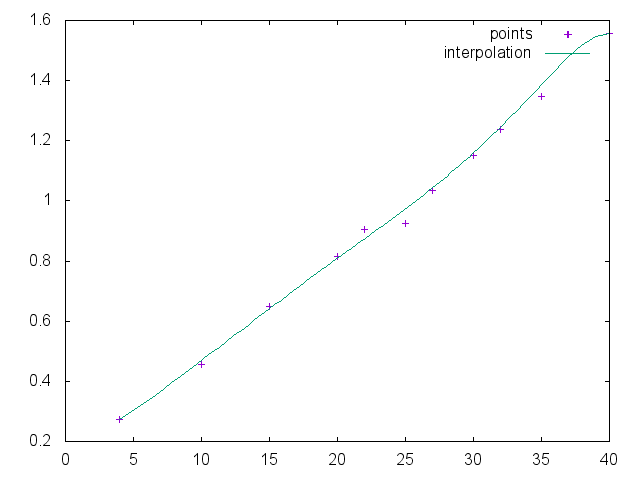
\includegraphics[width=\textwidth]{simpleheur}
\end{center}



\subsection{Relativní chyba}

Heuristika počítá rychleji, ale ač není úplně hloupá, dopouští se chyby, protože nevyzkouší všechny možnosti. 
Tuto chybu jsem spočítal po každé jednotlivé instanci pomocí vzorečku $( C(OPT)-C(APX) ) / C(OPT)$.
Po každé sadě instancí jsem chybu zprůměroval. Výsledky jsou v následující tabulce:

\begin{center}
\begin{tabular}{|c|c|}
\hline
Počet věcí & Relativní chyba \\
\hline\hline
4 & 0.0719 \\
\hline
10 & 0.0309 \\
\hline
15 & 0.0097 \\
\hline
20 & 0.0139 \\
\hline
22 & 0.0157 \\
\hline
25 & 0.0133 \\
\hline\hline
celkový průměr & 0.0259 \\
\hline
\end{tabular}
\end{center}

Po vynesení hodnot do grafu není na první pohled jasné,
jestli existuje nějaký jednoduchý vztah mezi počtem věcí a relativní chybou:

\begin{center}
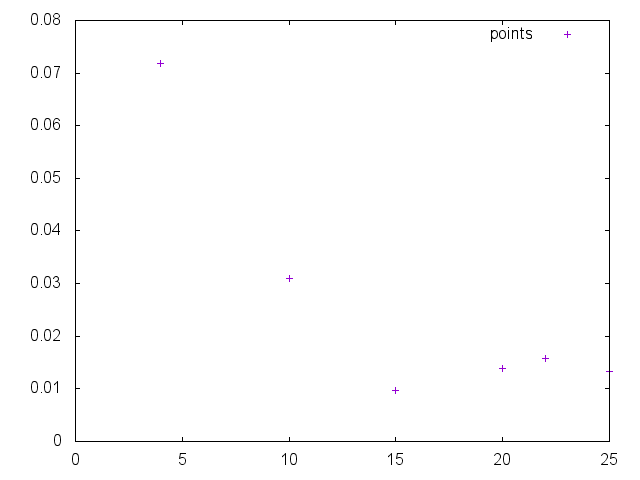
\includegraphics[width=\textwidth]{simpleheur_relerr}
\end{center}




\section{Závěr}

Je očividné, že heuristika způsobuje obrovské zrychlení. Oproti zdá se exponenciálnímu růstu potřebného času
u hrubé síly je vztah času a počtu věcí u heuristiky více méně lineární.

Relativní chyba vypadá, že bude možná s přibývajícími věcmi klesat. To ale nemusí být nutně pravda. Potřebovali bychom
větší počty věcí, jenže pro ty trvá hrubá síla extrémně dlouho.

\section{Přílohy}

\begin{description}
\item[sources.zip] Obsahuje balík zdrojových kódú v jazyce C. Neobsahuje makefile.
\end{description}



\end{document}